\frame{
\frametitle{\secname}

\begin{columns}
\column{0.6\textwidth}
\begin{itemize}
\item Division by $a$?
\begin{itemize}
\item If $a$ coprime with $m$, then $a\cdot a^{-1}=1$ exists
\end{itemize}
\item Exponentiation?
\begin{itemize}
\item $1,a,a^2,\dots,a^x,\dots\mod m$ will eventually repeat (pigeonhole)
\item If $a^{-1}$ exists, first repetition happens at $a^n=1$ ($n$ is the \emph{order} of $a$)
\end{itemize}
\item This is number theory!
\item Can't teach all of number theory in 1h
\item But useful for cryptography, etc.
\end{itemize}

\column{0.4\textwidth}
\begin{figure}
\centering
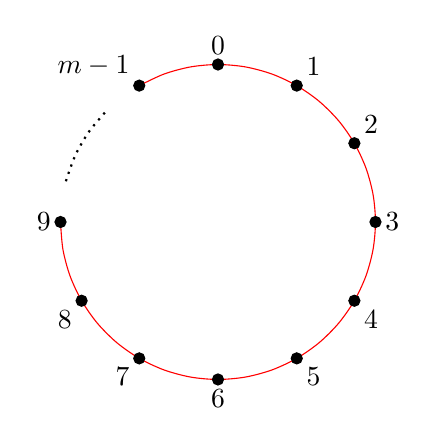
\begin{tikzpicture}
\def\r{2}
\draw[color=red,smooth,every node/.style={color=black},mark=*,mark size=2pt,mark options={color=black}]
    plot[domain=-30:270,samples=31,mark repeat=3] ({\r*cos(90-\x)},{\r*sin(90-\x)});
\draw[dotted,thick,smooth,every node/.style={color=black},mark=]
    plot[domain=285:315,samples=4] ({\r*cos(90-\x)},{\r*sin(90-\x)});
\node[above] (0) at (90:\r) {0};
\node[above right] (1) at (60:\r) {1};
\node[above right] (2) at (30:\r) {2};
\node[right] (2) at (0:\r) {3};
\node[below right] (2) at (-30:\r) {4};
\node[below right] (2) at (-60:\r) {5};
\node[below] (2) at (-90:\r) {6};
\node[below left] (2) at (-120:\r) {7};
\node[below left] (2) at (-150:\r) {8};
\node[left] (2) at (-180:\r) {9};
\node[above left] (3) at (120:\r) {$m-1$};
\end{tikzpicture}
\end{figure}

\end{columns}

}